\documentclass[conference]{IEEEtran}
\usepackage{cite}
\usepackage{amsmath,amssymb,amsfonts}
\usepackage{graphicx}
\usepackage{textcomp}
\usepackage{xcolor}
\usepackage{url}
\usepackage{tikz}
\usetikzlibrary{arrows.meta,calc}

% Photo and screenshot placeholders. Save the real image under the file name
% shown in the placeholder, in the same folder as this .tex file, and the
% next compile swaps the grey box for the image. No other edit is needed.
\newcommand{\shotfig}[3]{%
  \IfFileExists{#1}{\includegraphics[width=\columnwidth]{#1}}{%
    \fbox{\parbox[c][#2][c]{\dimexpr\columnwidth-2\fboxsep-2\fboxrule\relax}{%
      \centering\scriptsize\color{gray}#3}}}}

\begin{document}

\title{Industrial Worker Safety Monitoring and Emergency Alert System Using the NXP FRDM-RW612 Edge Platform}

% TODO(author): replace the bracketed placeholders with your real details.
% Add further authors (for example the project guide) with additional
% \and \IEEEauthorblockN{...} \IEEEauthorblockA{...} blocks.
\author{\IEEEauthorblockN{Yajnesh C B}
\IEEEauthorblockA{\textit{Dept. of Electronics and Communication Engineering} \\
\textit{[College name]}\\
{[City]}, {[Country]} \\
{[email address]}}
}

\maketitle

\begin{abstract}
Industrial workers face falls, hazardous gases, high temperatures and sudden emergencies, yet common safety practice depends on manual reporting or on standalone instruments that do not report their alarms. This paper describes a worker safety monitoring node built on the NXP FRDM-RW612 board, which pairs an Arm Cortex-M33 microcontroller with integrated Wi-Fi and Bluetooth Low Energy (BLE) radios. The node reads the onboard digital temperature sensor, an external MPU-6050 motion sensor and an MQ-2 gas sensor, and it treats the onboard user button as a manual emergency (SOS) input. Sensors are polled every 100 ms, and falls are recognized by a two-stage free-fall and impact rule. Firmware on the microcontroller classifies every sample as normal, warning or emergency and drives three light-emitting diodes (LEDs) and a buzzer without waiting for any network response. It also assembles telemetry packets and holds them in a small ring buffer while the link is down. A Flask-based laptop dashboard shows the node state, the readings and an event log, and its simulation controls let a demonstrator trigger each hazard. The prototype is built on a breadboard and powered over USB. The gas input and the wireless link run in simulation mode, so no packet yet reaches the dashboard from the board, and field accuracy has not been measured. The system is a functional academic prototype and not a certified safety device.
\end{abstract}

\begin{IEEEkeywords}
edge computing, emergency alerting, fall detection, industrial Internet of Things, worker safety
\end{IEEEkeywords}

\section{Introduction}
Manufacturing plants, workshops, warehouses and processing units expose workers to accidental falls, extreme ambient temperatures and flammable or toxic gases. The time between a hazardous event and the first response often decides the outcome, and surveys of industrial wearables show that continuous monitoring of workers and their surroundings is now a major research topic \cite{svertoka2021}.

Current practice falls into three groups. Manual reporting and periodic patrols depend on human vigilance and react after the fact. Standalone instruments, such as a single gas detector, sound a local alarm but do not tell anyone else. Centralized monitoring systems report to a server, but their sensing nodes lose the safety function when the wireless link fails. None of these combines detection on the device with automatic reporting over a network. Edge computing, which processes data close to its source to shorten response time and reduce bandwidth use \cite{shi2016}, points to a middle route: decide on the device, alert locally, and report whenever a link exists.

This paper describes a prototype that follows that route on the NXP FRDM-RW612 board. It contributes a four-stage node architecture, the on-device decision logic with its thresholds and alert patterns, a telemetry path with an offline queue, a Flask dashboard with simulation controls, a description of the breadboard build, and an account of which modules run on real hardware and which still run in simulation. Section~\ref{sec:related} reviews related work, Section~\ref{sec:architecture} gives the architecture, Section~\ref{sec:hardware} the hardware, Section~\ref{sec:firmware} the firmware logic, Section~\ref{sec:wireless} the wireless path, Section~\ref{sec:dashboard} the dashboard, Section~\ref{sec:build} the prototype build, Section~\ref{sec:status} the prototype status, Section~\ref{sec:limits} the limitations and Section~\ref{sec:conclusion} the conclusion.

\section{Related Work}
\label{sec:related}
Threshold-based fall detection on the resultant acceleration of a tri-axial sensor is a long-standing technique. Bourke et al.\ separated simulated falls from activities of daily living in a set of 480 movements with a single threshold on a trunk-mounted sensor \cite{bourke2007}. Reviews of fall detection point out that performance in real-life conditions, power consumption and real-time operation remain open problems \cite{igual2013}. The prototype in this paper adopts a threshold rule on the resultant acceleration and adds a free-fall stage before the impact test, which is a common way to reject sudden movements that are not falls. It also combines the fall rule with temperature, gas and manual inputs on one node, and it keeps local alerting independent of the wireless link.

\section{System Architecture}
\label{sec:architecture}
The node follows a four-stage pipeline of acquisition, edge decision, local alerting through light-emitting diodes (LEDs) and a buzzer, and wireless reporting, as shown in Fig.~\ref{fig:arch}. The FRDM-RW612 board \cite{nxpboard} is the central unit. It reads its onboard P3T1755 temperature sensor \cite{p3t1755}, an external MPU-6050 accelerometer and gyroscope \cite{mpu6050}, an external MQ-2 gas sensor \cite{mq2}, and the SW2 user button used as the emergency (SOS) input. The board is powered and debugged from a laptop over USB Type-C.

\begin{figure}[!t]
\centering
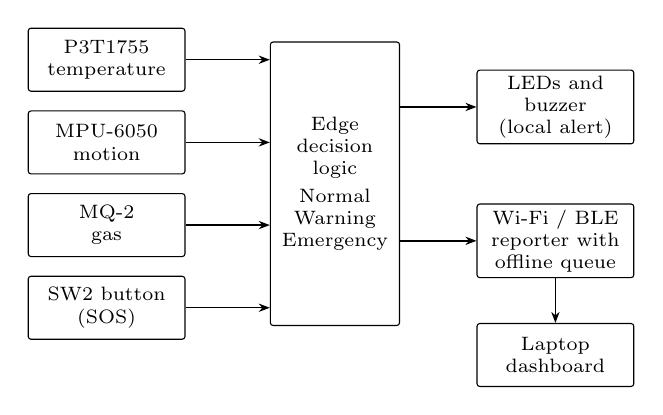
\begin{tikzpicture}[
  font=\scriptsize,
  blk/.style={draw, rounded corners=1pt, align=center, minimum height=0.8cm, text width=1.85cm, inner sep=2pt},
  arr/.style={-{Stealth[length=4pt]}, line width=0.5pt}
]
\node[blk] (temp) at (0,0) {P3T1755\\temperature};
\node[blk] (mpu) at (0,-1.05) {MPU-6050\\motion};
\node[blk] (gas) at (0,-2.1) {MQ-2\\gas};
\node[blk] (sos) at (0,-3.15) {SW2 button\\(SOS)};
\node[blk, minimum height=3.6cm, text width=1.5cm] (dec) at (2.9,-1.575) {Edge decision logic\\[2pt] Normal\\Warning\\Emergency};
\node[blk] (leds) at (5.7,-0.6) {LEDs and buzzer\\(local alert)};
\node[blk] (wifi) at (5.7,-2.3) {Wi-Fi / BLE\\reporter with\\offline queue};
\node[blk] (dash) at (5.7,-3.75) {Laptop\\dashboard};
\foreach \n in {temp,mpu,gas,sos}
  \draw[arr] (\n.east) -- (\n.east -| dec.west);
\draw[arr] (dec.east |- leds.west) -- (leds.west);
\draw[arr] (dec.east |- wifi.west) -- (wifi.west);
\draw[arr] (wifi.south) -- (dash.north);
\end{tikzpicture}
\caption{Block diagram of the worker safety node. Sensing, the decision and the local alert all run on the FRDM-RW612, and only the reporter depends on the wireless link.}
\label{fig:arch}
\end{figure}

Table~\ref{tab:hazards} lists how each hazard is detected and how the node responds locally, with gas limits given in parts per million (ppm). Every hazard also produces a status packet for the dashboard. When the link is down, local alerting carries on and the packets wait in a queue.

\begin{table}[!t]
\caption{Hazard rules and local response}
\label{tab:hazards}
\centering
\begin{tabular}{|p{0.55in}|p{1.1in}|p{1.3in}|}
\hline
\textbf{Hazard} & \textbf{Edge rule} & \textbf{Local response} \\
\hline
Fall & Resultant acceleration below 0.4 g, then above 2.5 g within 1.0 s & Emergency: red LED, pulsed buzzer, held for 5 s \\
\hline
Temperature & Warning at 40 \textdegree C or above, emergency at 50 \textdegree C or above & Warning: yellow LED, short chirp. Emergency: red LED, pulsed buzzer \\
\hline
Gas & Warning at 300 ppm or above, emergency at 600 ppm or above & Same as temperature \\
\hline
Manual SOS & SW2 pressed (active low) & Emergency at once, highest priority \\
\hline
\end{tabular}
\end{table}

\section{Hardware Implementation}
\label{sec:hardware}

\subsection{Board and Sensors}
The RW612 microcontroller on the FRDM-RW612 has an Arm Cortex-M33 core and Wi-Fi 6, Bluetooth Low Energy (BLE) 5.3 and IEEE 802.15.4 radios \cite{nxpboard}. The firmware sets the core clock to 260 MHz. The P3T1755 returns a 12-bit two's complement temperature with a resolution of 0.0625 \textdegree C per step, and the driver reads it over the inter-integrated circuit (I$^2$C) bus at address 0x48. The MPU-6050 sits at address 0x68 and is configured for a full scale of $\pm$2 g on the accelerometer and $\pm$250 degrees per second on the gyroscope. The MQ-2 analog output feeds channel 0 of the 12-bit low-power analog-to-digital converter (LPADC) on general-purpose input/output (GPIO) pin 60, with a 3.3 V reference. Its heater runs from the 5 V rail, and the module is suited to demonstrating gas detection but is not a certified industrial gas detector.

\subsection{Actuators and Pin Assignment}
Three 5 mm LEDs in green, yellow and red with 220 $\Omega$ series resistors show the node state, and an active buzzer module with its own driver transistor gives the audible alarm. Table~\ref{tab:pins} gives the pin assignment used by the firmware. The two I$^2$C devices share one bus, which is possible because their addresses differ. The debug console uses the MCU-Link virtual serial port at 115200 baud.

% VERIFY(author): board.h puts the MPU-6050 on Flexcomm 2 (GPIO 16/17), while
% docs/pinout_mapping.md, README.md and the card label in dashboard_app.py say
% Flexcomm 0 (GPIO 0/1). Keep this table in line with the wiring that is
% actually on your breadboard, and make the other three files agree with it.
\begin{table}[!t]
\caption{Pin assignment}
\label{tab:pins}
\centering
\begin{tabular}{|p{1.25in}|p{1.05in}|p{0.6in}|}
\hline
\textbf{Function} & \textbf{Interface} & \textbf{GPIO} \\
\hline
P3T1755 SDA, SCL & Flexcomm 2, I$^2$C & 16, 17 \\
\hline
MPU-6050 SDA, SCL & Flexcomm 2, I$^2$C & 16, 17 \\
\hline
MQ-2 output & LPADC channel 0 & 60 \\
\hline
SW2 (SOS) & Digital input & 24 \\
\hline
Buzzer & Digital output & 4 \\
\hline
Green, yellow, red LED & Digital output & 5, 6, 7 \\
\hline
Debug serial TX, RX & Flexcomm 3 & 26, 27 \\
\hline
\end{tabular}
\end{table}

\section{Firmware and Edge Decision Logic}
\label{sec:firmware}

\subsection{Execution Model}
The firmware is a single bare-metal loop. Each pass reads the three sensors, evaluates the safety state, updates the LEDs and buzzer, assembles a telemetry packet, and then waits 100 ms. The loop period is therefore the 100 ms delay plus the execution time of one pass. The SW2 level is read on every pass.

Each I$^2$C driver retries a failed transfer up to three times and rejects values outside the rated range of the sensor. Five consecutive failed reads set a fault flag in the driver. The decision logic skips any sample that is marked invalid.

\subsection{Fall Detection}
The resultant acceleration is
\begin{equation}
a = \sqrt{a_x^{2} + a_y^{2} + a_z^{2}},
\label{eq:mag}
\end{equation}
where $a_x$, $a_y$ and $a_z$ are the axis readings in units of g. A resting sensor reads about 1 g. When $a$ in \eqref{eq:mag} falls below 0.4 g, the logic treats the worker as in free fall and arms a window of ten loop passes, which is about 1.0 s. If $a$ rises above 2.5 g while the window is open, the logic reports a fall, enters the emergency state and holds it for 50 passes (about 5 s). A new free-fall sample restarts the window.

\subsection{Temperature and Gas Rules}
A temperature of 40 \textdegree C or more gives a warning, and 50 \textdegree C or more gives an emergency. The MQ-2 driver converts the 12-bit count $N$ to a concentration with the linear bring-up relation
\begin{equation}
c = \max\!\left(10,\; \frac{1000\,N}{4095}\right)\ \text{ppm},
\label{eq:gas}
\end{equation}
so under \eqref{eq:gas} the 300 ppm and 600 ppm thresholds correspond to counts of about 1229 and 2457. This mapping is an approximation. It is not the resistance-ratio curve of the datasheet \cite{mq2}, and it has not been calibrated against a reference gas.

\subsection{Priority and Alert Patterns}
The checks run in a fixed order: SOS first, then a latched or new fall, then temperature, then gas. An emergency from any check ends the evaluation at once. A temperature warning can still be raised to an emergency by a gas emergency, but a gas warning never replaces a temperature warning. Alerting follows the resulting state. In the normal state the green LED is on and the buzzer is silent. In the warning state the yellow LED is on and the buzzer chirps for 200 ms once per second. In the emergency state the red LED is on and the buzzer pulses with 100 ms on and 100 ms off. These outputs are driven directly from the evaluation result and do not use the wireless stack.

\section{Wireless Reporting and Offline Queue}
\label{sec:wireless}
Each pass assembles a packet with a message identifier, a timestamp, the safety state, the primary hazard, the temperature, the gas concentration, the resultant acceleration and an SOS flag. In the normal and warning states one packet is sent per second. In the emergency state a packet is sent on every pass, that is, about every 100 ms.

If the link is down, packets go into a ring buffer of 16 entries, and new packets are dropped once it is full. After the link returns, the firmware releases one buffered packet per pass. The firmware configuration names a laptop-hosted network, WorkerSafety\_AP, and a dashboard server on port 5000. In the present code the link manager only simulates these states, and the send functions update counters without opening a connection, so no packet leaves the board (Section~\ref{sec:status}).

\section{Monitoring Dashboard}
\label{sec:dashboard}

\subsection{Server and Interfaces}
The dashboard is a Python Flask application that serves one web page and three JavaScript Object Notation (JSON) endpoints, listed in Table~\ref{tab:endpoints}. It listens on port 5000 on all network interfaces of the laptop. The telemetry endpoint reads the packet identifier, temperature, acceleration, state and hazard fields of a packet. From the state it sets the LED and buzzer indicators, and it adds a log entry for every warning or emergency packet. The gas and SOS fields of a packet are not read yet.

\begin{table}[!t]
\caption{Dashboard routes}
\label{tab:endpoints}
\centering
\begin{tabular}{|p{1.0in}|p{0.45in}|p{1.4in}|}
\hline
\textbf{Route} & \textbf{Method} & \textbf{Purpose} \\
\hline
\texttt{/} & GET & Dashboard page \\
\hline
\texttt{/api/status} & GET & Current state as JSON, polled by the page every 800 ms \\
\hline
\texttt{/api/telemetry} & POST & Packet from the node \\
\hline
\texttt{/api/simulate} & POST & Demonstration event from a button \\
\hline
\end{tabular}
\end{table}

\subsection{Operator View}
The page opens with a banner that turns green, amber or red with the node state, the hazard and the time of the last update. Under the banner, three cards show the temperature, the resultant acceleration with its three axis components, and the gas concentration. The temperature and gas cards state their warning thresholds, and the gas badge changes at 300 ppm and 600 ppm. A fourth card mirrors the green, yellow and red LEDs and the buzzer and shows the packet counters. A log panel lists the latest fifteen events, newest first.

\subsection{Simulation Controls}
A control card has five buttons that call the simulation endpoint. They inject a manual SOS, a fall with a 2.85 g impact, a temperature of 48.5 \textdegree C, a gas level of 550 ppm, and a reset to the normal state. The SOS and fall events set the emergency state. The temperature and gas events set the warning state, which agrees with the thresholds in Table~\ref{tab:hazards}. With these buttons a demonstrator can show every screen state without the board.

Two behaviors of the present code limit what the screens show. In the normal state the status endpoint adds small random variation around nominal values and raises the packet counter on every poll, so the readings and the counter in that state do not come from the board. The page also receives nothing from the board until the Wi-Fi path is connected.

\subsection{Dashboard Views}
Fig.~\ref{fig:dash-normal}, Fig.~\ref{fig:dash-warn} and Fig.~\ref{fig:dash-emerg} show the dashboard in the normal, warning and emergency states. % TODO(author): confirm how each screenshot was produced (simulation button or a posted packet) and say so here.

\begin{figure}[!t]
\centering
\shotfig{fig_dashboard_normal.png}{6.2cm}{[Placeholder] Dashboard screenshot, normal state.\\File: fig\_dashboard\_normal.png}
\caption{Dashboard in the normal state.}
\label{fig:dash-normal}
\end{figure}

\begin{figure}[!t]
\centering
\shotfig{fig_dashboard_warning.png}{6.2cm}{[Placeholder] Dashboard screenshot, warning state (high temperature or gas).\\File: fig\_dashboard\_warning.png}
\caption{Dashboard in the warning state after a high-temperature event.}
\label{fig:dash-warn}
\end{figure}

\begin{figure}[!t]
\centering
\shotfig{fig_dashboard_emergency.png}{6.2cm}{[Placeholder] Dashboard screenshot, emergency state (SOS or fall) with the event log visible.\\File: fig\_dashboard\_emergency.png}
\caption{Dashboard in the emergency state after a fall event, with the event log.}
\label{fig:dash-emerg}
\end{figure}

\section{Prototype Build}
\label{sec:build}

\subsection{Components and Assembly}
Table~\ref{tab:bom} lists the parts of the breadboard prototype. The FRDM-RW612 takes its power from the laptop over USB Type-C, so the build needs no battery, charger or external temperature sensor. Without the laptop, the parts cost roughly INR 3,300 to 4,000. % TODO(author): confirm the cost range against your receipts.

\begin{table}[!t]
\caption{Components of the breadboard prototype}
\label{tab:bom}
\centering
\begin{tabular}{|p{1.35in}|p{0.35in}|p{1.2in}|}
\hline
\textbf{Component} & \textbf{Qty} & \textbf{Purpose} \\
\hline
FRDM-RW612 board & 1 & Controller, radios, onboard temperature sensor \\
\hline
MPU-6050 (GY-521) module & 1 & Motion and fall detection \\
\hline
MQ-2 gas sensor module & 1 & Gas hazard demonstration \\
\hline
Active buzzer module & 1 & Audible alarm \\
\hline
5 mm LEDs (green, yellow, red) & 3 & State indication \\
\hline
220 $\Omega$ resistors & 3 & LED current limiting \\
\hline
Breadboard and jumper wires & 1 set & Circuit assembly \\
\hline
USB Type-C cable & 1 & Power, programming, debugging \\
\hline
Laptop & 1 & Programming, console, dashboard \\
\hline
\end{tabular}
\end{table}

All parts sit on one breadboard beside the board, as shown in Fig.~\ref{fig:proto}. The MPU-6050 module runs from the 3.3 V rail and the MQ-2 heater from the 5 V rail, and all grounds are common. The MPU-6050 uses the I$^2$C pins in Table~\ref{tab:pins}, and the MQ-2 analog output goes to the LPADC pin. Each LED has its own 220 $\Omega$ resistor. The buzzer module has its own driver transistor, so a GPIO pin can drive it directly.

\begin{figure}[!t]
\centering
\shotfig{fig_prototype.jpg}{6.2cm}{[Placeholder] Photo of the assembled breadboard prototype.\\File: fig\_prototype.jpg}
\caption{Breadboard prototype of the worker safety node with the FRDM-RW612, the MPU-6050, the MQ-2 module, three LEDs and the buzzer.}
\label{fig:proto}
\end{figure}

\subsection{Bench Setup and Demonstration}
The same USB cable programs the board and carries the debug console through the onboard MCU-Link probe. During development the state, hazard, fall count, packet counters and sensor values are watched in the debugger, and the console prints one line per second with the temperature, the three acceleration axes and the gas value. The dashboard runs on the same laptop.

Each hazard can be exercised on the bench. Pressing SW2 raises the SOS. A fall needs a reading below 0.4 g followed by one above 2.5 g, which a sharp movement of the MPU-6050 module can produce. The simulation levels of the gas driver stand in for a leak, and a manual warning flag in the debugger forces the warning state in place of a real temperature rise. The link manager's simulated reconnect after 3 s exercises the offline queue. % TODO(author): confirm that this is how you triggered each case, and edit the paragraph to match what you actually did.

\section{Prototype Status}
\label{sec:status}
Table~\ref{tab:status} summarizes what runs on the board and what runs in simulation. The temperature and motion drivers, the decision logic, the LEDs, the buzzer and the SOS input are implemented against real hardware registers. The MQ-2 driver has a simulation mode with a normal level and two leak levels, and the LPADC read is not yet connected. The link manager simulates a connected state and a reconnect after 30 passes (3 s), so the queue and flush path is exercised without a radio. The send functions only update counters, so the dashboard is fed by its own simulation controls at present.

\begin{table}[!t]
\caption{Module status in the present prototype}
\label{tab:status}
\centering
\begin{tabular}{|p{1.3in}|p{1.75in}|}
\hline
\textbf{Module} & \textbf{Status} \\
\hline
P3T1755 driver & Implemented, with retries and range check \\
\hline
MPU-6050 driver & Implemented, with identity check \\
\hline
MQ-2 driver & Simulation mode, linear conversion \\
\hline
Decision logic, LEDs, buzzer, SOS & Implemented \\
\hline
Wi-Fi link & Simulated link state \\
\hline
Telemetry and offline queue & Implemented over the simulated link; no packet leaves the board \\
\hline
Flask dashboard & Implemented, with simulation controls; normal-state readings simulated \\
\hline
\end{tabular}
\end{table}

Because the loop reads every input once per pass, a temperature, gas or SOS condition is seen on the next pass, so its detection delay is bounded by one loop period plus the execution time of a pass, which is slightly more than 100 ms. This is a design bound, and no measurement backs it yet. % TODO(author): add measured latency, fall-detection sensitivity and specificity, and power figures here once you have logged them, with the test method.

\section{Limitations and Future Work}
\label{sec:limits}
The MQ-2 responds to several gases and drifts with temperature and humidity, so it can demonstrate the concept but cannot support a certified gas alarm. The present accelerometer setup, with a $\pm$2 g range, a 5 Hz digital low-pass filter and 10 Hz polling, limits how well a short impact peak above 2.5 g can be captured. Raising the range and the sampling rate, and reading the sensor outside the delay loop, is the first planned change. The driver fault flags are not yet turned into a warning on the node, so a failed sensor currently drops out of the decision silently. The wireless transport is still simulated, BLE is not yet used, and a 16-entry queue holds only a few seconds of normal traffic. The dashboard shows simulated values in the normal state, ignores the gas and SOS fields of a packet and has no authentication on its endpoints. Fall detection, gas calibration and latency have not been measured on a test population or with reference equipment.

Planned extensions follow the project scope: a cloud-connected platform for several workers, location tracking with GPS or indoor positioning, certified industrial sensors, a battery-powered wearable form factor and low-power operating modes.

\section{Conclusion}
\label{sec:conclusion}
The prototype shows that a single FRDM-RW612 board can read temperature, motion, gas and an SOS button, classify the worker's condition on the device, and sound a local alarm with no network involved. The same board assembles telemetry for a Flask dashboard, whose simulation controls reproduce each alert state, and holds packets in a 16-entry queue while the link is down. The build is a breadboard powered over USB. The temperature, motion, SOS and alert paths run on real hardware, while the gas input and the wireless link are still simulated, so measured accuracy and latency remain the next step.

\begin{thebibliography}{00}
\bibitem{svertoka2021} E. Svertoka et al., ``Wearables for industrial work safety: A survey,'' \textit{Sensors}, vol. 21, no. 11, Art. no. 3844, Jun. 2021, doi: 10.3390/s21113844.
\bibitem{shi2016} W. Shi, J. Cao, Q. Zhang, Y. Li, and L. Xu, ``Edge computing: Vision and challenges,'' \textit{IEEE Internet Things J.}, vol. 3, no. 5, pp. 637--646, Oct. 2016.
\bibitem{bourke2007} A. K. Bourke, J. V. O'Brien, and G. M. Lyons, ``Evaluation of a threshold-based tri-axial accelerometer fall detection algorithm,'' \textit{Gait Posture}, vol. 26, no. 2, pp. 194--199, Jul. 2007.
\bibitem{igual2013} R. Igual, C. Medrano, and I. Plaza, ``Challenges, issues and trends in fall detection systems,'' \textit{BioMed. Eng. OnLine}, vol. 12, Art. no. 66, 2013.
\bibitem{nxpboard} NXP Semiconductors, ``FRDM-RW612 Wi-Fi development board,'' product documentation. [Online]. Available: \url{https://www.nxp.com/design/design-center/development-boards-and-designs/FRDM-RW612}
% TODO(author): add revision and date to the three data-sheet references below.
\bibitem{p3t1755} NXP Semiconductors, ``P3T1755 digital temperature sensor,'' data sheet.
\bibitem{mpu6050} InvenSense, ``MPU-6000 and MPU-6050 product specification,'' Rev. 3.4, Aug. 2013.
\bibitem{mq2} Winsen Electronics, ``MQ-2 semiconductor sensor for combustible gas,'' data sheet.
\end{thebibliography}

\end{document}
